\noindent\textbf{Islr2 is a cell surface LRR-domain-containing receptor expressed by retinal ganglion cells.}\newline
\indent In order to identify putative novel regulators of midline crossing in zebrafish, we assembled a catalogue of all annotated LRR receptors listed by the zebrafish model organism database, ZFIN \cite{bradford2011zfin}, starting from the collection of mammalian orthologs for these proteins \cite{dolan2007extracellular}.
Within our dataset of 116 genes, we identified 23 receptors expressed in the zebrafish RGC layer that we hypothesized may play a role in retinal axon guidance.
Because we are interested in cellular recognition events at the midline, we focused our attention on receptor-encoding genes that are expressed in RGCs between 30 and 36 h, the time between the beginning of RGC differentiation and chiasm establishment.
Most genes (e.g. \emph{ntrk2b}, \emph{lrrc4.1}, \emph{flrt1a}, \emph{lrtm2}) were expressed at later stages (48 hpf onwards), leaving a single candidate, \emph{islr2}, fulfilling the temporal expression pattern suitable for further study.
In general, \emph{islr2} is expressed in brain nuclei associated with differentiated neurons (Figure~\ref{Linxfig1}A), similar to descriptions of mouse and chick \emph{Islr2} expression \cite{gejima2006lrr,homma2009expression}.
The dynamic pattern of \emph{islr2} transcription and its correlation with the birthdate of RGCs are suggestive of a postdifferentiation function held by this protein.
Because \emph{islr2} expression starts in the very first cohort of RGCs developing in the retina (Figure~\ref{Linxfig1}A), we hypothesized that Islr2 might be involved in early guidance decisions that these cells take, such as midline crossing.
\begin{figure}[hbtp]
    \begin{center}
        \includegraphics{Figures/Linx_fig1.pdf}
        \caption[Zebrafish \emph{islr2} is expressed in RGCs and is necessary for complete retinal axon midline crossing.]
        {Zebrafish \emph{islr2} is expressed in RGCs and is necessary for complete retinal axon midline crossing.
		A) Time-course of \emph{islr2} mRNA expression in zebrafish embryos and larvae.
		At 36 hpf, when the optic chiasm is established, \emph{islr2} is in RGCs (arrowheads).
		At 48 hpf the RGC layer is evenly populated by neurons expressing \emph{islr2}.
		At 72 hpf there is a slight decrease in \emph{islr2} mRNA level and a subset of \emph{islr2}\textsuperscript{+} amacrine cells.
		Dashed outlines highlight retinas.
		Upper row: ventral view.
		Lower row: lateral view.
		Anterior is at left.
		B) Schematic of \emph{islr2\textsuperscript{sa82}} TILLING allele.
		The mutant ORF haa a premature stop codon, leading to truncation of the LRR-CT domain.
		C) \emph{islr2} mutant larvae have ipsilateral retinal projections.
		First row: dorsal view of wild-type larva at 5 dpf.
		The optic nerves from each eye cross the midline to innervate the contra optic tectum (dashed lines).
		Rows 2-3: two homozygote mutant animals, displaying ectopic innervation of the ipsi tectum (asterisks).
		The larva in row 2 also shows a thinner optic nerve (arrow) than the individual in row 3.
		All pictures are dorsal views, maximum intensity projections of confocal Z-stacks.
		Anterior is at left.
		Scale=50$\mu$m.
		D) Relationship between optic nerve width (brackets) and ipsi misrouting of axons (arrowheads) at the chiasm of \emph{islr2} mutant larvae.
		Homozygous mutant individuals with normal optic nerve (second column) display a higher number of ipsilateral fibers, compared to mutants with thinner nerves.
		Single optical sections.
		Ventral views.
		Anterior is at top.
		ON: optic nerve.
		Scale=50$\mu$m. 
		D$'$) Phenotype distribution in \emph{islr2} mutants compared to siblings from two clutches.
		Mutant larvae (black bars) have a higher number of ectopic neurites in the ipsi tectum, compared to controls (grey bars) and to larvae with thinner optic nerves (compare to D$''$).
		Innervation of contra tectum was unaffected in mutants compared to siblings.
		CL: contralateral.
		D$''$) Analysis of two clutches where larvae with thinner nerves were identified.
		Only a subset of mutant animals (black bars) display ipsi innervation of the tectum, while in many mutants these neurites are undetectable, likely because of extreme reduction in axon number.
		In most mutant animals, innervation of the contra tectum is reduced, suggesting that thinning of the optic nerve and ipsi projections are independent phenotypes.
		CL: contralateral.
		}
        \label{Linxfig1}
    \end{center}
\end{figure}

\noindent\textbf{Islr2 is necessary for retinal axon midline crossing in zebrafish.}\newline
\indent To investigate the function of Islr2 \invivo{}, we selected a zebrafish mutant strain harboring a germline mutation in \emph{islr2}, generated by TILLING.
The \emph{islr2\textsuperscript{sa82}} locus contains a premature nonsense mutation that leads to a protein truncation before the end of the LRR domain (Figure~\ref{Linxfig1}B).
As a consequence, this allele is expected to behave as a functional null.

To score for phenotypes related to retinal axon guidance, we anterogradely labeled the optic nerves by intraretinal lipophilic dye injections at 5 dpf, at which time this axon tract is stable, since most error correction events have terminated by 72 hpf \cite{hutson2002pathfinding} and robust visual behaviors are displayed by wild-type larvae \cite{easter1996development,neuhauss2003behavioral}.
Strikingly, despite being mostly normal morphologically, \emph{islr2} homozygous mutant larvae clearly display ipsilaterally-projecting retinal axons (Figure~\ref{Linxfig1}C, asterisks).
We also observed that a subset of \emph{islr2} mutants had thinner optic nerves compared to wild-type siblings (arrow in Figure~\ref{Linxfig1}C, D).
The ipsilateral projection phenotype is fully penetrant in larvae with normal optic nerve width, but varies in expressivity, ranging from just a few misprojecting axons to significant innervation of the ipsilateral optic tectum (asterisks in Figure~\ref{Linxfig1}C, D$'$).
In cases where the optic nerve was hypoplastic, the extent of ipsilateral innervation was also reduced (Figure~\ref{Linxfig1}C, D$''$).
This array of phenotypes indicated that the guidance effect of Islr2 could be uncoupled from a putative trophic role of this receptor (described in \citenoparens{mandai2009lig}), which would not, however, be specific for the retinal axon projection.
We therefore focused further investigation on the axon pathfinding defects we detected.

To characterize the behavior of misprojecting axons during embryonic and early larval development, we labeled the retinal projection of \emph{islr2} mutants at different stages.
Mutant axons slightly lag behind the rates of axon extension observed in wild-type siblings at 40 and 48 hpf and growth cones with a spread-out morphology could be recognized in the midline region (Figure~\ref{Linxfig2}).
From 48 hpf, it was possible to follow ipsilaterally growing axons from the chiasm (arrow and arrowheads in Figure~\ref{Linxfig2}).
Accordingly, 5 dpf larvae from the same clutch presented different levels of ipsilateral innervation of the optic tectum (asterisks in Figure~\ref{Linxfig2}), sometimes associated with optic nerve hypoplasia.
\begin{figure}[hbtp]
    \begin{center}
        \includegraphics{Figures/Linx_fig2.pdf}
        \caption[Chronological progression of the \emph{islr2\textsuperscript{-/-}} phenotype.]
        {Chronological progression of the \emph{islr2\textsuperscript{-/-}} phenotype.
		Anterogradely-labeled retinal projections of \emph{islr2} mutant embryos and larvae compared to control siblings.
		At 40 and 48 hpf growth cones can be observed in the proximity of the midline in mutant embryos, while these seem to have proceeded to the optic tract in wild-type siblings.
		Additionally, axonal extension defects can be recognized in mutants compared to controls (40 hpf, 48 hpf, 72 hpf, \emph{islr2\textsuperscript{-/-}}, first column).
		From 48 hpf, ipsilateral neurites (arrow) are visible in mutant embryos and can be traced back to the chiasm.
		As expected, 5 dpf mutant larvae displayed ectopic innervation of the ipsilateral optic tectum (asterisks).
		At this stage, \emph{islr2\textsuperscript{-/-}} larvae show misrouted fibers at the chiasm (arrowheads).
		All pictures are maximum intensity projections of confocal Z-stacks.
		Anterior is to the top.
		Scale=50$\mu$m.
		}
        \label{Linxfig2}
    \end{center}
\end{figure}

In addition to their apparently normal morphology, \emph{islr2} mutant larvae do not present widespread axon guidance defects (Figure~\ref{Linxfig3}A).
Sections through the plane of the optic chiasm showed unaffected layered retinal structure (Figure~\ref{Linxfig3}B) and morphologically normal ventral diencephalic tissue (Figure~\ref{Linxfig3}C).
Collectively, these data led us to hypothesize that Islr2 function is specifically required in RGCs.
Also, because a cohort of axons misproject ipsilaterally at the chiasm in mutants (arrowheads in Figure~\ref{Linxfig2}), we conclude that Islr2 is required for correct midline crossing of RGC axons and not for their guidance to the optic tectum in zebrafish.
\begin{figure}[hbtp]
    \begin{center}
        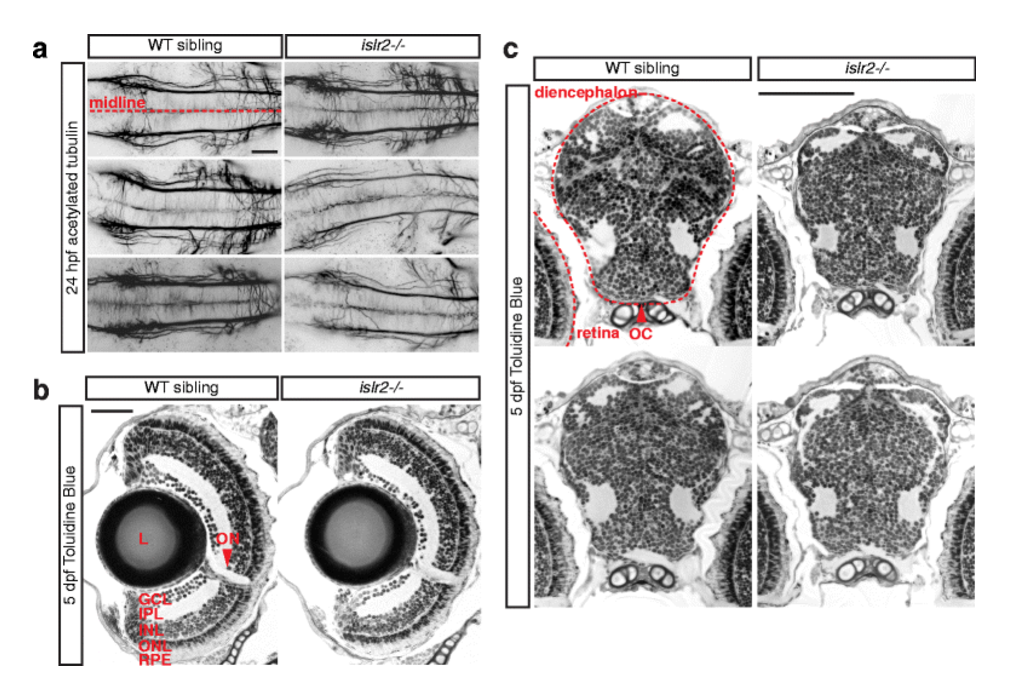
\includegraphics{Figures/LinxFig3.pdf}
        \caption[Zebrafish \emph{islr2} mutants do not display widespread axon guidance defects and are morphologically normal.]
        {Zebrafish \emph{islr2} mutants do not display widespread axon guidance defects and are morphologically normal.
		a) Acetylated tubulin staining of 24 hpf embryos showing central axon tracts at the level of the medial longitudinal fasciculus (MLF).
		Thinner axon bundles were observed only in a subset of \emph{islr2} mutant animals.
		The general spacing and directionality of nerve fibers was unaltered compared to controls, indicating absence of guidance defects in these axons.
		Maximum intensity projections of confocal Z-stacks.
		Dorsal views.
		Anterior is to the left.
		Scale=50$\mu$m.
		b) Transverse sections through the retina of 5 dpf \emph{islr2} mutants.
		Normal size, gross anatomy and layering of the retina were observed in \emph{islr2} mutants.
		RGC number may be decreased in some \emph{islr2\textsuperscript{-/-}} larvae.
		L: lens.
		GCL: ganglion cell layer.
		IPL: inner plexiform layer.
		INL: inner nuclear layer.
		ONL: outer nuclear layer.
		RPE: retinal pigmented epithelium.
		ON: optic nerve.
		Scale=50$\mu$m.
		c) Transverse sections at the level of the optic chiasm in \emph{islr2} mutants and siblings.
		The chiasmatic and ventral diencephalic tissue appear normal in size and patterning, suggesting that the axon guidance phenotype of \emph{islr2} larvae does not originate from mispatterning effects.
		OC: optic chiasm.
		Scale=100$\mu$m.
}
        \label{Linxfig3}
    \end{center}
\end{figure}

\noindent\textbf{\emph{Islr2} mutant mice display retinal axon defects at the optic chiasm.}\newline
\indent We examined \emph{Islr2} mutant mice (\emph{Linx\textsuperscript{tEGFP}} mice; \cite{mandai2009lig}) to further explore the role of \emph{Islr2} in the decussation decisions of retinal axons navigating the optic chiasm.
Islr2 is expressed by RGCs in the mouse retina (\citenoparens{blackshaw2004genomic} and data not shown), and RGC axons in mutant mice misroute at the optic chiasm and along the optic tract (Figure~\ref{LinxMsFig}).
A greater number of retinal axons aberrantly re-enter the contralateral optic nerve in \emph{Islr2} mutants (Figure~\ref{LinxMsFig}B,C) compared to heterozygous (Figure~\ref{LinxMsFig}A) and wild-type (not shown) littermates.
The mutant optic chiasm also appears widened rostrocaudally relative to the heterozygote chiasm region (Figure~\ref{LinxMsFig}A-C).
Although \emph{Islr2} mutant mice do not directly recapitulate the ipsilateral projection phenotype found in zebrafish, there are marked errors in axon routing in both the proximal and distal optic tract in \emph{Islr2} mutants.
Bundles of axons defasciculate from the rest of the optic tract on both ipsi- and contralateral sides of the chiasm (Figure~\ref{LinxMsFig}B,C, high power of contralateral defasciculation in Figure~\ref{LinxMsFig}B$'$,C$'$), and farther along the tract we detected several axons prematurely leaving the tract and entering the medial thalamus (Figure~\ref{LinxMsFig}A$''$-C$''$).
The common element in the axon routing errors in the mouse and the zebrafish mutants is a lack of coherence of RGC axons, whether at the chiasm or farther along their pathway in the tract.
This array of axon routing defects in \emph{Islr2} mutant mice further supports a role for \emph{Islr2} in fostering axon bundle coherence and proper tract formation, in response to axon guidance cues at the midline and along the optic tract.
\begin{figure}[hbtp]
    \begin{center}
        \includegraphics[width=\textwidth]{Figures/LinxMsFig.pdf}
        \caption[Loss of Islr2 leads to axon routing errors at the optic chiasm and tract in mice.]
        {Loss of Islr2 leads to axon routing errors at the optic chiasm and tract in mice.
		E16.5 \emph{Islr2} mutant mice display expanded chiasms along the antero-posterior axis (brackets in B and C, compared to A).
		In addition, a greater number of axons enter the opposite optic nerve with retinopetal directionality (arrows in B and C).
		Although no clear increase in the number of ipsilaterally-projecting fibers relative to the contralateral projection can be observed, other defects were identified along the post-crossing route of RGC axons.
		Defasciculation effects in the optic tract were observed both at ventral (B$'$ and C$'$)and dorsal locations (B$''$ and C$''$), where many axons stray from their normal course (arrowheads).
		Arrowheads in B$'$ and C$'$ indicate axons departing rostrally from the chiasm, a common phenotype observed in situations when guidance through the chiasm is impaired. 
		I: ipsilateral.
		C: contralateral.
		ON: optic nerve.
		OC: optic chiasm.
		OT: optic tract.
		Scale=500$\mu$m (A-C), 200$\mu$m (A$'$-C$'$ and A$''$-C$''$).
		}
        \label{LinxMsFig}
    \end{center}
\end{figure}

\noindent\textbf{Discussion}\newline
\indent Cell surface and secreted proteins are fundamental mediators of axon guidance, especially because they dictate how growth cones interface with the environment during navigation.
The identification of novel receptor-ligand pairs controlling axon directionality, however, is complicated by the existence of accessory molecules that modify the interactions between cognate receptors and ligands and by the transiency of interactions mediated
by these molecules.
This typical feature of membrane proteins is essential for regulating dynamic functions during nervous system development, but obfuscates both the identification of related phenotypes and their recapitulation \exvivo{}.
In the context of retinal axon pathfinding in zebrafish, even unbiased discovery strategies, such as large-scale forward genetic screens, have resulted in the isolation of very few guidance receptors acting cell-autonomously in misrouted axons \cite{karlstrom1996zebrafish,trowe1996mutations}.
In fact, the majority of mutants showing defects in the laterality of the retinal projection also display mispatterning of the ventral midline tissue, suggesting that local tissue architecture in the ventral diencephalon is critical for the actuation of midline crossing \cite{barresi2005hedgehog,seth2006belladonna,bergeron2011brother}.
Therefore, genetic approaches to dissect redundant biological processes suffer from intrinsic limitations and might require the utilization of sensitized mutant backgrounds.

Here we have used the zebrafish as a model for the decision of RGC axons to cross the midline, a process common to the ontogeny of the visual pathway in all animals \cite{jeffery2005variations}.
To overcome the constraints of genetic analysis mentioned above, we took a candidate approach by screening the zebrafish repertoire of cell surface LRR molecules, known modulators of axon pathfinding.
We spatiotemporally compared the available gene expression patterns with the steps in axon growth leading to the formation of the retinal projection in zebrafish.
The expression dynamics of our final candidate, \emph{islr2}, correlate with the timing of RGC generation and chiasm establishment.
\emph{Islr2} knockout mice display striking neuronal defects, including thinning and increased branching of sensory and motor limb projections \cite{mandai2009lig} and complete absence of the internal capsule \cite{mandai2014linx}.
However, while \emph{Islr2} expression in RGCs is shared in zebrafish, chick \cite{gejima2006lrr}, and mouse \cite{blackshaw2004genomic}, nothing was known about the functional role of \emph{Islr2} in the visual system.
Here we demonstrate that Islr2 controls axon routing at the zebrafish and mouse optic chiasm.

Axons of both the optic nerve and of central longitudinal tracts can appear decreased in number in zebrafish \emph{islr2} mutants.
To understand whether this phenotype is due to disrupted intraretinal axon guidance, we used an RGC-specific \emph{isl2b:GFP} transgenic line \cite{pittman2008pathfinding} and did not detect ectopic neurites in mutant retinas (data not shown).
As an alternative explanation, newly differentiated RGCs could be susceptible to higher rates of apoptosis in mutant embryos.
In agreement with results from mouse Islr2 mutants \cite{mandai2009lig}, \emph{islr2/tp53} double mutants do not rescue \emph{islr2\textsuperscript{-/-}} defects in fish (data not shown).
These results leave lack of trophic support as a candidate explanation for the optic nerve hypoplasia observed in \emph{islr2} mutants.
Although consistent with a described role of Islr2 in modulating neurotrophin and GDNF/Ret signaling \cite{mandai2009lig}, this phenotype was not fully penetrant.

Data shown here implicate a novel LRR receptor, Islr2, in retinal axon guidance in zebrafish and mouse.
\emph{Islr2} larvae with normally populated optic nerves display an ectopic ipsilateral retinal projection originating from the chiasm.
In addition, \emph{Islr2} mutant mice present a similar phenotype of straying axons caudal to the midline, misrouting of axons into the opposite optic nerve, and manifest a widening of the chiasm.
These results reveal a function for Islr2 in controlling RGC axon guidance and coherence through the optic chiasm, in conjunction with trophic support in the retina, across species.

One of the zebrafish Islr2 binding partners, Vasnb, is specifically expressed by cells anterior to the optic chiasm.
We hypothesize that these cells belong to the glial knot and mediate midline crossing of zebrafish retinal axons along the ventral diencephalon, as they are the primary cell type contacted by RGC axons extending through the chiasm.
These results highlight the redundant signaling environment at the optic chiasm, orchestrating axon guidance choices to cross or avoid the midline, all the while maintaining coherent bundles as axons project to their targets.